\chapter{Introduction}
\label{chapter:introduction}

\begin{introduction}
    "The only source of knowledge is experience." - Albert Einstein
\end{introduction}



\section{Internship Context and Framework}

This document represents the final report of the internship carried out as part of the Internship Curricular Unit (49991) of the second year of studies of the Master's Degree in Clinical Bioinformatics, with specialization in Genome Bioinformatics, at the University of Aveiro. The internship lasted nine months, starting on November 21st, 2023, and ending on July 19th, 2024, totalling 1296 hours of work. 

During this period, the trainee had the opportunity to apply the knowledge acquired throughout the course and to get involved in practical projects related to bioinformatics and genomics. Unilabs, a recognized company in the health area, provided a professional environment where the intern could collaborate with experienced professionals and actively participate in projects relevant to clinical bioinformatics. This report addresses the activities developed during the internship and the contributions to the projects in which the intern was involved. 

This introductory section aims to offer an overview of the context in which the internship was carried out, laying the foundations for understanding the activities and results presented throughout the report.


\section{Project motivation and objectives }

Currently, Unilabs uses a genomic intelligence platform that uses natural language processing to analyse new scientific publications of a genetic nature and incorporate them into an always updated knowledge base. This platform is particularly useful in prioritizing sequenced variants, for genetic diagnosis purposes, in their interpretation and in the production of clinical reports, thus enabling the provision of increasingly personalized care. 

However, at the time of this internship, Unilabs was in the migration phase to this new platform and, therefore, as a complementary strategy, a new independent software was developed to obtain the necessary metrics for genomic analyses, not directly provided by the aforementioned platform, ensuring compliance with the guidelines and practices recommended for Next Generation Sequencing (NGS). These metrics are important for assessing data quality, i.e., they indicate how well the target regions were covered by sequencing. In the case of the present stage, it was suggested to obtain the sequencing depth. In addition, the depth of coverage directly influences the ability to detect genetic variants: regions with low coverage can result in undetected or underestimated variants. Additionally, coverage metrics are also useful to optimize sequencing protocols, adjusting experimental parameters to ensure adequate coverage of target regions and minimize unnecessary costs. 

As will be explained in detail below, the software created and described in this report allows the obtaining of Average Read Depth and Percentage of Coverage at 1x, 10x, 15x, 20x, 30x, 50x, 100x, and 500x per gene and per panel in analysis of gene panels. Additionally, in addition to the presentation of metrics by panel, single gene and exome analysis was also implemented.

\section{Document Structure}
This document is divided into five chapters, each with several sections. 

The first chapter, the Introduction, begins with a contextualization and framing of the internship carried out, followed by a brief presentation of the motivation and objectives of the work. The host entity is also described, in addition to a brief theoretical foundation that supports the solution presented. 

The second chapter, Analysis Tool, includes several sections. The first is Development, which explains the bioinformatic process involved in the creation of the software, including the configuration of the work environment, the programming languages and software used, and the calculations performed. The following section, Operation, details step-by-step how the software operates to obtain the desired metrics. The Validation section compares the metrics obtained by the software with other tools. Next, the Documentation section describes the process of documenting the software to ensure its reproducibility. Finally, the Distribution section explains how software can be distributed and deployed. 

The third chapter, Discussion, is intended to debate the ideas associated with the work, analysing and interpreting the results in the context of existing knowledge in the area. It emphasizes possible practical applications, limitations, and implications of the results. 

The last two chapters are, respectively, Final Considerations, where possible improvements and new features for future versions of the software are presented, and Bibliography, which lists all the sources consulted and cited in the work.

\section{Characterization of the Host Entity and Work Plan}
\subsection{Unilabs Portugal}

Since the beginning of 2006, Unilabs has established solid roots in Portugal. It began its journey with the acquisition of most of the shares of the company "Medicina Laboratorial Dr. Carlos Torres" and since then it has grown steadily, following a strategy of acquiring high-quality laboratories and partners throughout the country. 

It has more than 3,500 employees and more than 500 doctors, and operates in more than 1,000 service units, performing more than 25 million medical procedures per year. 

In 2017, Unilabs took an important step by acquiring BASE Holding. With this acquisition, it has expanded its service offering to include radiology, affirming its position as a national leader in integrated clinical diagnostics and the provision of Complementary Diagnostic and Therapeutic Means. 

Currently, it offers a wide variety of services in various areas, including Clinical Analysis, Pathological Anatomy, Cardiology, Gastroenterology, Medical Genetics, Nuclear Medicine and Radiology. The company maintains its commitment to being close to people, providing answers that contribute to a healthier future. \cite{unilabs_sobre}

\subsection{Unilabs Genetics}
Unilabs Genetics (formerly called CGC Genetics) was founded three decades ago and was the first private Medical Genetics laboratory in Portugal. It has been present on the national scene regarding diagnosis through genetic studies. It has a wide selection of tests and is known for its collaborative and thorough approach, meeting the demands of clinicians in a variety of specialist areas. 

It is a leader in Europe in Medical Genetics, with special emphasis on rare diseases. It provides accurate diagnoses for public and private healthcare institutions, providing physicians and patients with detailed information about the nature of diseases, prognosis, and treatment options. In addition, the company supports academic institutions, research centres and the pharmaceutical industry with data and knowledge that contributes to the discovery of biomarkers and the development of new drugs. 

The Unilabs Genetics laboratory is located in the city of Porto and combines advanced technologies, bioinformatics and artificial intelligence, with a highly qualified team of medical geneticists, specialists in genetic counselling and laboratory technicians. The company follows the strictest quality and ethics policies, having certifications (CLIA, ISO 15189, ISO 9001) that guarantee excellence in its services. \cite{unilabs_genetica}
\subsection{Schedule}

\begin{figure}[H]
    \centering
    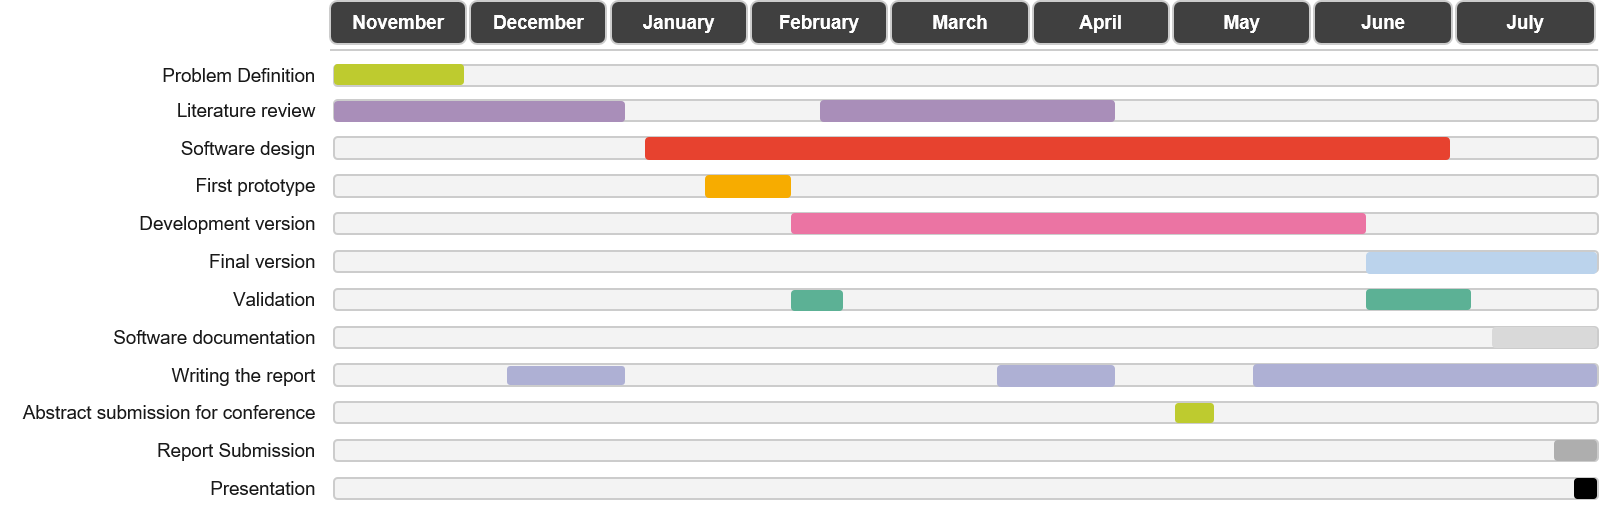
\includegraphics[width=1\textwidth]{figs/schedule.png}
    \caption{Imagem provisória do cronograma do estágio.}
    \label{fig:timeline}
\end{figure}

\section{Theoretical Framework}
\subsection{Evolution of genetics over the year}

The history of genetics formally began in 1865 with Gregor Mendel's work on plant hybridization. However, the term "genetics" was only coined in 1906 by the English biologist William Bateson to define the new science of heredity. Based on Mendel's laws, genetics introduced groundbreaking concepts such as gene, genotype, and phenotype. By the 1910s, Mendelian genetics merged with the chromosomal theory of inheritance, giving rise to classical genetics. In this framework, the gene was seen as a unit of function, transmission, recombination, and mutation. \cite{genetictimeline2}

This understanding persisted until the 1950s, when DNA was discovered as the material basis of heredity, marking the start of molecular biology. \cite{Gayon2016}

Following the discovery of DNA as hereditary material, molecular biology began to uncover the complexity of gene function. The fusion of Mendel's ideas with chromosomal theory also provided a more tangible understanding of genes, which could now be physically located on chromosomes. This integration led to significant advances, such as explaining Mendel's laws through cellular mechanisms and discovering genetic recombination. Genetics evolved into a more institutionalized science, with the establishment of academic chairs and specialized courses worldwide, solidifying its position as a central field in the biological sciences. \cite{Gayon2016}

The emergence of genomics in the latter half of the 20th century further transformed the field of genetics. The completion of the Human Genome Project in 2003 \cite{Collins1995}, a milestone in genomics, revealed the entire sequence of human DNA, propelling the study of genes beyond individual units to entire genomes. This large-scale approach allowed scientists to explore the intricate network of genes and their interactions, significantly advancing our understanding of complex traits and diseases. Genomics also facilitated the development of personalized medicine, where treatments could be tailored based on an individual's genetic makeup. \cite{Gayon2016}

The discovery of the RNA-guided CRISPR-Cas9 system has made genome editing easier and more efficient. This breakthrough allows scientists to modify DNA in various cells and organisms with ease, removing previous experimental barriers. Today, CRISPR-Cas9 is widely used in basic research, biotechnology, and the development of new therapies. \cite{CRISPR-CAS9}

Figure \ref{fig:timeline} presents a timeline with some of the major historical milestones in the evolution of genetics over the years.

\begin{figure}[H]
    \centering
    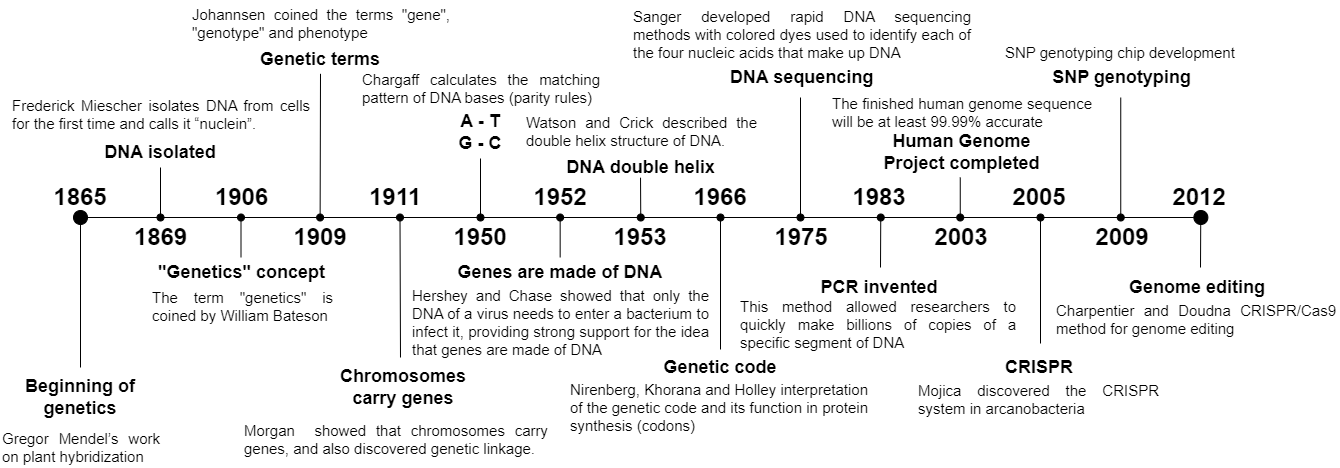
\includegraphics[width=1\textwidth]{figs/timeline.png}
    \caption{Evolution of genetics over the years: A brief timeline with some of the major historical milestones. Image adapted from \cite{genetictimeline} and \cite{genetictimeline2}}
    \label{fig:timeline}
\end{figure}

\subsection{Genetics vs Genomics}

Genetics and genomics are both fields of study that explore the roles of genes in living organisms, but they focus on different aspects of heredity and DNA. Genetics is the study of specific genes and their influence on traits and conditions that are passed from one generation to the next. It examines how certain genes cause inherited disorders, such as cystic fibrosis and Huntington's disease. \cite{NHGRI2018}

In contrast, genomics is a more recent field that encompasses the study of all the genes within an organism, referred to as the genome, and how these genes interact with each other and the environment. Unlike genetics, which focuses on individual genes, genomics uses advanced technologies like bioinformatics and high-performance computing to analyze vast amounts of genetic data. This comprehensive approach is crucial for studying complex diseases, such as cancer and diabetes, which result from the interplay between multiple genes and environmental factors. While both fields contribute to advancements in health and disease treatment, genomics represents a broader, more holistic view of genetic influence. \cite{JAX2017}

\subsection{Structure and function of DNA, RNA, and proteins}

Nucleic acids, specifically deoxyribonucleic acid (DNA) and ribonucleic acid (RNA), are fundamental molecules in biological systems, playing key roles in storing and transmitting genetic information. DNA, which exists primarily as a double-stranded helix, encodes the instructions necessary for the growth, development, and reproduction of all living organisms. RNA, on the other hand, serves multiple purposes, including acting as a messenger that carries genetic information from DNA to the ribosomes for protein synthesis. The structural complexity and functional versatility of these molecules underscore their importance in the central dogma of molecular biology, which describes the flow of genetic information from DNA to RNA to proteins. \cite{Minchin2019}

\subsection{Molecular Structure of DNA}

The molecular structure of DNA is a polymer composed of repeating units called nucleotides. Each nucleotide consists of three components: a five-carbon sugar (deoxyribose), a phosphate group, and a nitrogenous base. The nitrogenous bases are categorized into two groups: purines (adenine and guanine) and pyrimidines (cytosine and thymine). The nucleotides are linked together by phosphodiester bonds, forming a sugar-phosphate backbone that gives DNA its structural integrity. DNA molecules are double-stranded, with two complementary strands running in opposite directions (antiparallel orientation). These strands are held together by hydrogen bonds between specific base pairs: adenine pairs with thymine, and guanine pairs with cytosine. This complementary base pairing is crucial for the accurate replication and transmission of genetic information. \cite{Minchin2019}

The Figure \ref{fig:DNA} shows a representation of the molecular structure of DNA and the base pairing between adenine (A), thymine (T), cytosine (C), and guanine (G).

\begin{figure}[H]
    \centering
    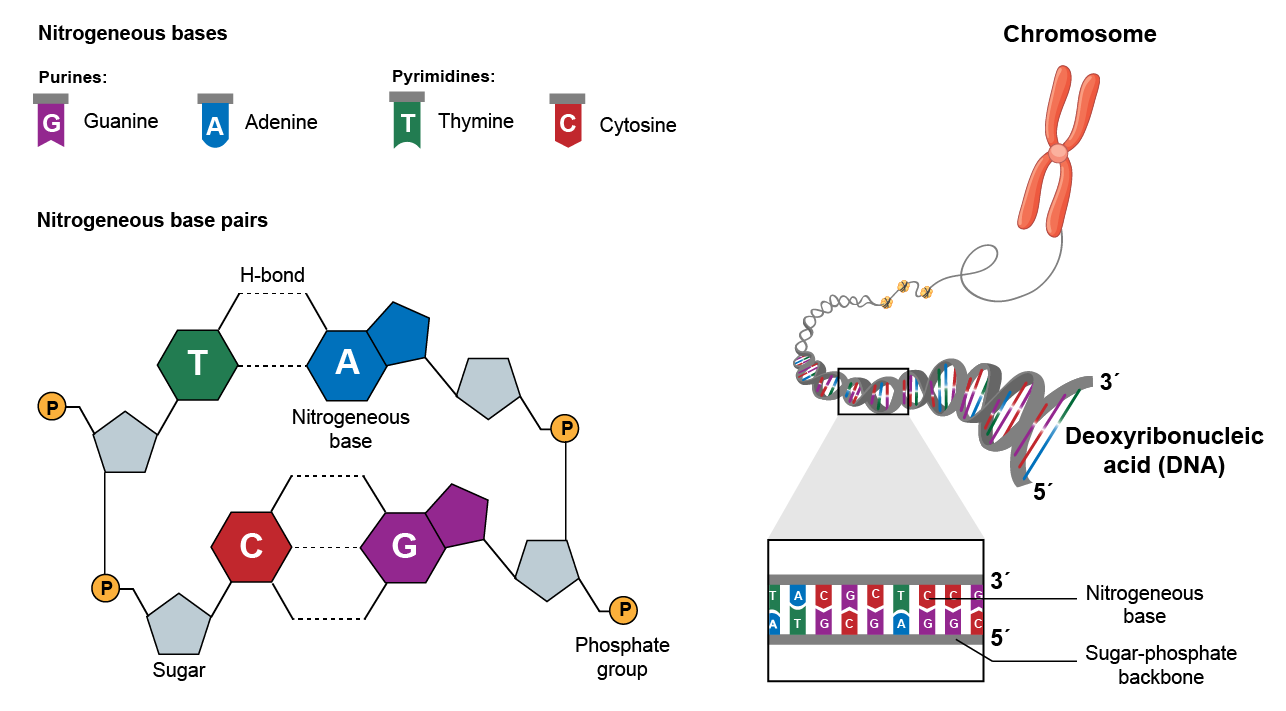
\includegraphics[width=1\textwidth]{figs/DNA.png}
    \caption{Representation of DNA and its constituents. In the top left corner, the nitrogenous bases are illustrated, categorized into Purines (Guanine and Adenine) and Pyrimidines (Thymine and Cytosine). Below this, on the left side, the paired nitrogenous bases are shown, along with their respective hydrogen bonds and the sugar-phosphate backbone connections. On the right side of the image, a chromosome is depicted unraveling, revealing the DNA structure. \cite{DNA}} 
    \label{fig:DNA}
\end{figure}

\subsection{Discovery of the Double Helix}

The three-dimensional structure of DNA, famously known as the double helix, was elucidated by James Watson and Francis Crick in 1953. Their discovery was informed by Rosalind Franklin’s X-ray diffraction images, which revealed the helical structure of DNA. Watson and Crick proposed that the two strands of the helix are wound around each other, with the sugar-phosphate backbone on the outside and the nitrogenous bases on the inside. The helical structure is right-handed, with ten base pairs per turn of the helix. The stability of the double helix is largely due to the hydrogen bonds between the complementary base pairs and the hydrophobic interactions between the stacked bases. This discovery not only explained how DNA could carry genetic information but also provided insights into how it could be replicated during cell division. \cite{Minchin2019}

\subsection{DNA Packaging in Eukaryotic Cells}

In eukaryotic cells, DNA is not free-floating within the nucleus; instead, it is highly organized and compacted into structures known as chromosomes. This compaction is achieved through the association of DNA with histone proteins, forming nucleosomes, which are the basic unit of chromatin. Each nucleosome consists of a segment of DNA wrapped around a core of histone proteins. These nucleosomes are further coiled and folded into higher-order structures, eventually forming the condensed chromosomes visible during cell division. The packaging of DNA into chromatin is essential for fitting the large eukaryotic genome into the limited space of the nucleus. Furthermore, chromatin structure plays a crucial role in gene regulation, as regions of tightly packed chromatin (heterochromatin) are generally transcriptionally inactive, while loosely packed regions (euchromatin) are more accessible to transcriptional machinery. \cite{Minchin2019}

\subsection{Mutations and genetic variations}

Mutations are fundamental drivers of genetic diversity, occurring when changes happen in the DNA sequence. These alterations can range from small-scale mutations, such as the substitution, insertion, or deletion of one or a few nucleotides, to large-scale mutations that involve significant chromosome segments or entire genes. Chromosome mutations specifically impact either individual nucleotides or larger chromosome fragments. They can involve deletions, insertions, inversions, translocations, or even gene duplications. On the other hand, genome mutations refer to changes in the number of whole chromosomes or sets of chromosomes and are studied separately. \cite{merrick2016}

Genetic variation, on the other hand, refers to the observable differences between individuals within a population, which arise from variations in their genotypes. While mutations are the source of new genetic variation, genetic variation encompasses the broader concept of how different alleles at specific loci contribute to diversity within a population. This variation is shaped and refined by evolutionary forces such as natural selection, gene flow, and genetic drift. In cultivated plants, human-directed selection can also manipulate genetic variation to enhance desirable traits. \cite{merrick2016}